% Created by tikzDevice version 0.12
% !TEX encoding = UTF-8 Unicode
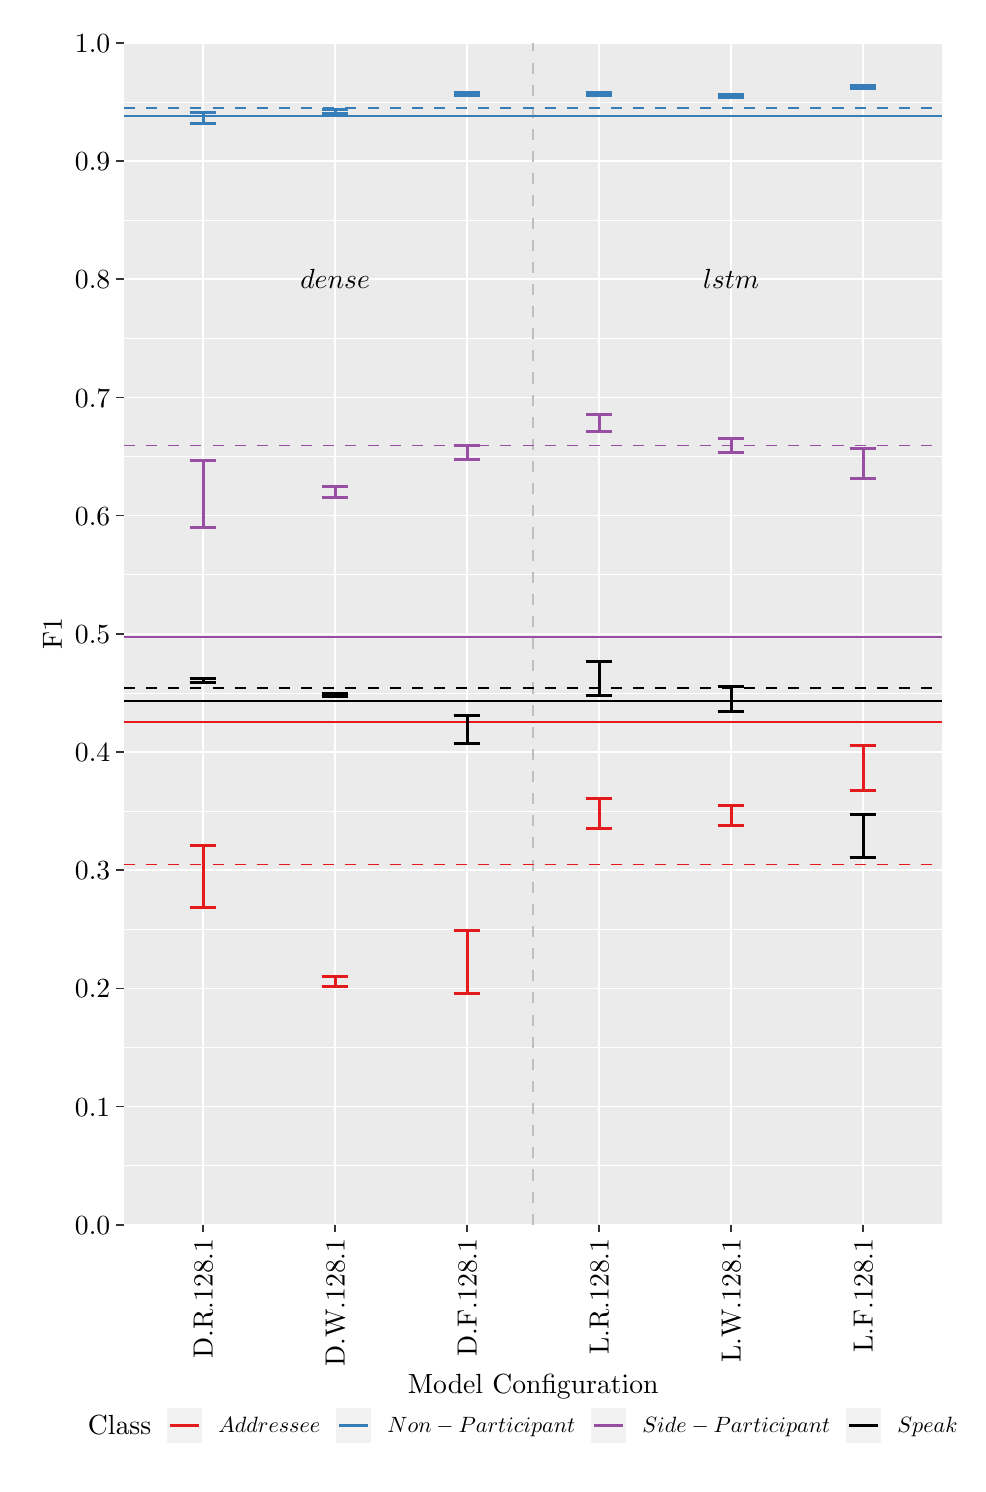
\begin{tikzpicture}[x=1pt,y=1pt]
\definecolor{fillColor}{RGB}{255,255,255}
\path[use as bounding box,fill=fillColor,fill opacity=0.00] (0,0) rectangle (336.00,519.12);
\begin{scope}
\path[clip] (  0.00,  0.00) rectangle (336.00,519.12);
\definecolor{drawColor}{RGB}{255,255,255}
\definecolor{fillColor}{RGB}{255,255,255}

\path[draw=drawColor,line width= 0.6pt,line join=round,line cap=round,fill=fillColor] (  0.00,  0.00) rectangle (336.00,519.12);
\end{scope}
\begin{scope}
\path[clip] ( 34.81, 86.52) rectangle (330.50,513.62);
\definecolor{fillColor}{gray}{0.92}

\path[fill=fillColor] ( 34.81, 86.52) rectangle (330.50,513.62);
\definecolor{drawColor}{RGB}{255,255,255}

\path[draw=drawColor,line width= 0.3pt,line join=round] ( 34.81,107.87) --
	(330.50,107.87);

\path[draw=drawColor,line width= 0.3pt,line join=round] ( 34.81,150.58) --
	(330.50,150.58);

\path[draw=drawColor,line width= 0.3pt,line join=round] ( 34.81,193.29) --
	(330.50,193.29);

\path[draw=drawColor,line width= 0.3pt,line join=round] ( 34.81,236.00) --
	(330.50,236.00);

\path[draw=drawColor,line width= 0.3pt,line join=round] ( 34.81,278.71) --
	(330.50,278.71);

\path[draw=drawColor,line width= 0.3pt,line join=round] ( 34.81,321.42) --
	(330.50,321.42);

\path[draw=drawColor,line width= 0.3pt,line join=round] ( 34.81,364.13) --
	(330.50,364.13);

\path[draw=drawColor,line width= 0.3pt,line join=round] ( 34.81,406.84) --
	(330.50,406.84);

\path[draw=drawColor,line width= 0.3pt,line join=round] ( 34.81,449.55) --
	(330.50,449.55);

\path[draw=drawColor,line width= 0.3pt,line join=round] ( 34.81,492.26) --
	(330.50,492.26);

\path[draw=drawColor,line width= 0.6pt,line join=round] ( 34.81, 86.52) --
	(330.50, 86.52);

\path[draw=drawColor,line width= 0.6pt,line join=round] ( 34.81,129.23) --
	(330.50,129.23);

\path[draw=drawColor,line width= 0.6pt,line join=round] ( 34.81,171.94) --
	(330.50,171.94);

\path[draw=drawColor,line width= 0.6pt,line join=round] ( 34.81,214.65) --
	(330.50,214.65);

\path[draw=drawColor,line width= 0.6pt,line join=round] ( 34.81,257.36) --
	(330.50,257.36);

\path[draw=drawColor,line width= 0.6pt,line join=round] ( 34.81,300.07) --
	(330.50,300.07);

\path[draw=drawColor,line width= 0.6pt,line join=round] ( 34.81,342.78) --
	(330.50,342.78);

\path[draw=drawColor,line width= 0.6pt,line join=round] ( 34.81,385.49) --
	(330.50,385.49);

\path[draw=drawColor,line width= 0.6pt,line join=round] ( 34.81,428.20) --
	(330.50,428.20);

\path[draw=drawColor,line width= 0.6pt,line join=round] ( 34.81,470.91) --
	(330.50,470.91);

\path[draw=drawColor,line width= 0.6pt,line join=round] ( 34.81,513.62) --
	(330.50,513.62);

\path[draw=drawColor,line width= 0.6pt,line join=round] ( 63.42, 86.52) --
	( 63.42,513.62);

\path[draw=drawColor,line width= 0.6pt,line join=round] (111.11, 86.52) --
	(111.11,513.62);

\path[draw=drawColor,line width= 0.6pt,line join=round] (158.81, 86.52) --
	(158.81,513.62);

\path[draw=drawColor,line width= 0.6pt,line join=round] (206.50, 86.52) --
	(206.50,513.62);

\path[draw=drawColor,line width= 0.6pt,line join=round] (254.19, 86.52) --
	(254.19,513.62);

\path[draw=drawColor,line width= 0.6pt,line join=round] (301.88, 86.52) --
	(301.88,513.62);
\definecolor{drawColor}{RGB}{190,190,190}

\path[draw=drawColor,line width= 0.6pt,dash pattern=on 4pt off 4pt ,line join=round] (182.65, 86.52) -- (182.65,513.62);
\definecolor{drawColor}{RGB}{0,0,0}

\node[text=drawColor,anchor=base,inner sep=0pt, outer sep=0pt, scale=  1.00] at (111.11,424.74) {\(dense\)};

\node[text=drawColor,anchor=base,inner sep=0pt, outer sep=0pt, scale=  1.00] at (254.19,424.74) {\(lstm\)};

\path[draw=drawColor,line width= 0.6pt,line join=round] ( 34.81,275.79) -- (330.50,275.79);
\definecolor{drawColor}{RGB}{55,126,184}

\path[draw=drawColor,line width= 0.6pt,line join=round] ( 34.81,487.24) -- (330.50,487.24);
\definecolor{drawColor}{RGB}{228,26,28}

\path[draw=drawColor,line width= 0.6pt,line join=round] ( 34.81,268.26) -- (330.50,268.26);
\definecolor{drawColor}{RGB}{152,78,163}

\path[draw=drawColor,line width= 0.6pt,line join=round] ( 34.81,299.02) -- (330.50,299.02);
\definecolor{drawColor}{RGB}{0,0,0}

\path[draw=drawColor,line width= 0.6pt,dash pattern=on 4pt off 4pt ,line join=round] ( 34.81,280.51) -- (330.50,280.51);
\definecolor{drawColor}{RGB}{55,126,184}

\path[draw=drawColor,line width= 0.6pt,dash pattern=on 4pt off 4pt ,line join=round] ( 34.81,490.16) -- (330.50,490.16);
\definecolor{drawColor}{RGB}{228,26,28}

\path[draw=drawColor,line width= 0.6pt,dash pattern=on 4pt off 4pt ,line join=round] ( 34.81,216.73) -- (330.50,216.73);
\definecolor{drawColor}{RGB}{152,78,163}

\path[draw=drawColor,line width= 0.6pt,dash pattern=on 4pt off 4pt ,line join=round] ( 34.81,368.15) -- (330.50,368.15);
\definecolor{drawColor}{RGB}{0,0,0}

\path[draw=drawColor,line width= 1.1pt,line join=round] ( 58.65,283.79) --
	( 68.19,283.79);

\path[draw=drawColor,line width= 1.1pt,line join=round] ( 63.42,283.79) --
	( 63.42,282.55);

\path[draw=drawColor,line width= 1.1pt,line join=round] ( 58.65,282.55) --
	( 68.19,282.55);

\path[draw=drawColor,line width= 1.1pt,line join=round] ( 58.65,283.79) --
	( 68.19,283.79);

\path[draw=drawColor,line width= 1.1pt,line join=round] ( 63.42,283.79) --
	( 63.42,282.55);

\path[draw=drawColor,line width= 1.1pt,line join=round] ( 58.65,282.55) --
	( 68.19,282.55);

\path[draw=drawColor,line width= 1.1pt,line join=round] ( 58.65,283.79) --
	( 68.19,283.79);

\path[draw=drawColor,line width= 1.1pt,line join=round] ( 63.42,283.79) --
	( 63.42,282.55);

\path[draw=drawColor,line width= 1.1pt,line join=round] ( 58.65,282.55) --
	( 68.19,282.55);

\path[draw=drawColor,line width= 1.1pt,line join=round] ( 58.65,283.79) --
	( 68.19,283.79);

\path[draw=drawColor,line width= 1.1pt,line join=round] ( 63.42,283.79) --
	( 63.42,282.55);

\path[draw=drawColor,line width= 1.1pt,line join=round] ( 58.65,282.55) --
	( 68.19,282.55);

\path[draw=drawColor,line width= 1.1pt,line join=round] ( 58.65,283.79) --
	( 68.19,283.79);

\path[draw=drawColor,line width= 1.1pt,line join=round] ( 63.42,283.79) --
	( 63.42,282.55);

\path[draw=drawColor,line width= 1.1pt,line join=round] ( 58.65,282.55) --
	( 68.19,282.55);

\path[draw=drawColor,line width= 1.1pt,line join=round] ( 58.65,283.79) --
	( 68.19,283.79);

\path[draw=drawColor,line width= 1.1pt,line join=round] ( 63.42,283.79) --
	( 63.42,282.55);

\path[draw=drawColor,line width= 1.1pt,line join=round] ( 58.65,282.55) --
	( 68.19,282.55);

\path[draw=drawColor,line width= 1.1pt,line join=round] ( 58.65,283.79) --
	( 68.19,283.79);

\path[draw=drawColor,line width= 1.1pt,line join=round] ( 63.42,283.79) --
	( 63.42,282.55);

\path[draw=drawColor,line width= 1.1pt,line join=round] ( 58.65,282.55) --
	( 68.19,282.55);

\path[draw=drawColor,line width= 1.1pt,line join=round] ( 58.65,283.79) --
	( 68.19,283.79);

\path[draw=drawColor,line width= 1.1pt,line join=round] ( 63.42,283.79) --
	( 63.42,282.55);

\path[draw=drawColor,line width= 1.1pt,line join=round] ( 58.65,282.55) --
	( 68.19,282.55);

\path[draw=drawColor,line width= 1.1pt,line join=round] (106.34,278.50) --
	(115.88,278.50);

\path[draw=drawColor,line width= 1.1pt,line join=round] (111.11,278.50) --
	(111.11,277.53);

\path[draw=drawColor,line width= 1.1pt,line join=round] (106.34,277.53) --
	(115.88,277.53);

\path[draw=drawColor,line width= 1.1pt,line join=round] (106.34,278.50) --
	(115.88,278.50);

\path[draw=drawColor,line width= 1.1pt,line join=round] (111.11,278.50) --
	(111.11,277.53);

\path[draw=drawColor,line width= 1.1pt,line join=round] (106.34,277.53) --
	(115.88,277.53);

\path[draw=drawColor,line width= 1.1pt,line join=round] (106.34,278.50) --
	(115.88,278.50);

\path[draw=drawColor,line width= 1.1pt,line join=round] (111.11,278.50) --
	(111.11,277.53);

\path[draw=drawColor,line width= 1.1pt,line join=round] (106.34,277.53) --
	(115.88,277.53);

\path[draw=drawColor,line width= 1.1pt,line join=round] (106.34,278.50) --
	(115.88,278.50);

\path[draw=drawColor,line width= 1.1pt,line join=round] (111.11,278.50) --
	(111.11,277.53);

\path[draw=drawColor,line width= 1.1pt,line join=round] (106.34,277.53) --
	(115.88,277.53);

\path[draw=drawColor,line width= 1.1pt,line join=round] (106.34,278.50) --
	(115.88,278.50);

\path[draw=drawColor,line width= 1.1pt,line join=round] (111.11,278.50) --
	(111.11,277.53);

\path[draw=drawColor,line width= 1.1pt,line join=round] (106.34,277.53) --
	(115.88,277.53);

\path[draw=drawColor,line width= 1.1pt,line join=round] (106.34,278.50) --
	(115.88,278.50);

\path[draw=drawColor,line width= 1.1pt,line join=round] (111.11,278.50) --
	(111.11,277.53);

\path[draw=drawColor,line width= 1.1pt,line join=round] (106.34,277.53) --
	(115.88,277.53);

\path[draw=drawColor,line width= 1.1pt,line join=round] (106.34,278.50) --
	(115.88,278.50);

\path[draw=drawColor,line width= 1.1pt,line join=round] (111.11,278.50) --
	(111.11,277.53);

\path[draw=drawColor,line width= 1.1pt,line join=round] (106.34,277.53) --
	(115.88,277.53);

\path[draw=drawColor,line width= 1.1pt,line join=round] (106.34,278.50) --
	(115.88,278.50);

\path[draw=drawColor,line width= 1.1pt,line join=round] (111.11,278.50) --
	(111.11,277.53);

\path[draw=drawColor,line width= 1.1pt,line join=round] (106.34,277.53) --
	(115.88,277.53);

\path[draw=drawColor,line width= 1.1pt,line join=round] (154.04,270.43) --
	(163.58,270.43);

\path[draw=drawColor,line width= 1.1pt,line join=round] (158.81,270.43) --
	(158.81,260.38);

\path[draw=drawColor,line width= 1.1pt,line join=round] (154.04,260.38) --
	(163.58,260.38);

\path[draw=drawColor,line width= 1.1pt,line join=round] (154.04,270.43) --
	(163.58,270.43);

\path[draw=drawColor,line width= 1.1pt,line join=round] (158.81,270.43) --
	(158.81,260.38);

\path[draw=drawColor,line width= 1.1pt,line join=round] (154.04,260.38) --
	(163.58,260.38);

\path[draw=drawColor,line width= 1.1pt,line join=round] (154.04,270.43) --
	(163.58,270.43);

\path[draw=drawColor,line width= 1.1pt,line join=round] (158.81,270.43) --
	(158.81,260.38);

\path[draw=drawColor,line width= 1.1pt,line join=round] (154.04,260.38) --
	(163.58,260.38);

\path[draw=drawColor,line width= 1.1pt,line join=round] (154.04,270.43) --
	(163.58,270.43);

\path[draw=drawColor,line width= 1.1pt,line join=round] (158.81,270.43) --
	(158.81,260.38);

\path[draw=drawColor,line width= 1.1pt,line join=round] (154.04,260.38) --
	(163.58,260.38);

\path[draw=drawColor,line width= 1.1pt,line join=round] (154.04,270.43) --
	(163.58,270.43);

\path[draw=drawColor,line width= 1.1pt,line join=round] (158.81,270.43) --
	(158.81,260.38);

\path[draw=drawColor,line width= 1.1pt,line join=round] (154.04,260.38) --
	(163.58,260.38);

\path[draw=drawColor,line width= 1.1pt,line join=round] (154.04,270.43) --
	(163.58,270.43);

\path[draw=drawColor,line width= 1.1pt,line join=round] (158.81,270.43) --
	(158.81,260.38);

\path[draw=drawColor,line width= 1.1pt,line join=round] (154.04,260.38) --
	(163.58,260.38);

\path[draw=drawColor,line width= 1.1pt,line join=round] (154.04,270.43) --
	(163.58,270.43);

\path[draw=drawColor,line width= 1.1pt,line join=round] (158.81,270.43) --
	(158.81,260.38);

\path[draw=drawColor,line width= 1.1pt,line join=round] (154.04,260.38) --
	(163.58,260.38);

\path[draw=drawColor,line width= 1.1pt,line join=round] (154.04,270.43) --
	(163.58,270.43);

\path[draw=drawColor,line width= 1.1pt,line join=round] (158.81,270.43) --
	(158.81,260.38);

\path[draw=drawColor,line width= 1.1pt,line join=round] (154.04,260.38) --
	(163.58,260.38);

\path[draw=drawColor,line width= 1.1pt,line join=round] (201.73,290.06) --
	(211.27,290.06);

\path[draw=drawColor,line width= 1.1pt,line join=round] (206.50,290.06) --
	(206.50,277.96);

\path[draw=drawColor,line width= 1.1pt,line join=round] (201.73,277.96) --
	(211.27,277.96);

\path[draw=drawColor,line width= 1.1pt,line join=round] (201.73,290.06) --
	(211.27,290.06);

\path[draw=drawColor,line width= 1.1pt,line join=round] (206.50,290.06) --
	(206.50,277.96);

\path[draw=drawColor,line width= 1.1pt,line join=round] (201.73,277.96) --
	(211.27,277.96);

\path[draw=drawColor,line width= 1.1pt,line join=round] (201.73,290.06) --
	(211.27,290.06);

\path[draw=drawColor,line width= 1.1pt,line join=round] (206.50,290.06) --
	(206.50,277.96);

\path[draw=drawColor,line width= 1.1pt,line join=round] (201.73,277.96) --
	(211.27,277.96);

\path[draw=drawColor,line width= 1.1pt,line join=round] (201.73,290.06) --
	(211.27,290.06);

\path[draw=drawColor,line width= 1.1pt,line join=round] (206.50,290.06) --
	(206.50,277.96);

\path[draw=drawColor,line width= 1.1pt,line join=round] (201.73,277.96) --
	(211.27,277.96);

\path[draw=drawColor,line width= 1.1pt,line join=round] (201.73,290.06) --
	(211.27,290.06);

\path[draw=drawColor,line width= 1.1pt,line join=round] (206.50,290.06) --
	(206.50,277.96);

\path[draw=drawColor,line width= 1.1pt,line join=round] (201.73,277.96) --
	(211.27,277.96);

\path[draw=drawColor,line width= 1.1pt,line join=round] (201.73,290.06) --
	(211.27,290.06);

\path[draw=drawColor,line width= 1.1pt,line join=round] (206.50,290.06) --
	(206.50,277.96);

\path[draw=drawColor,line width= 1.1pt,line join=round] (201.73,277.96) --
	(211.27,277.96);

\path[draw=drawColor,line width= 1.1pt,line join=round] (201.73,290.06) --
	(211.27,290.06);

\path[draw=drawColor,line width= 1.1pt,line join=round] (206.50,290.06) --
	(206.50,277.96);

\path[draw=drawColor,line width= 1.1pt,line join=round] (201.73,277.96) --
	(211.27,277.96);

\path[draw=drawColor,line width= 1.1pt,line join=round] (201.73,290.06) --
	(211.27,290.06);

\path[draw=drawColor,line width= 1.1pt,line join=round] (206.50,290.06) --
	(206.50,277.96);

\path[draw=drawColor,line width= 1.1pt,line join=round] (201.73,277.96) --
	(211.27,277.96);

\path[draw=drawColor,line width= 1.1pt,line join=round] (249.42,281.01) --
	(258.96,281.01);

\path[draw=drawColor,line width= 1.1pt,line join=round] (254.19,281.01) --
	(254.19,271.99);

\path[draw=drawColor,line width= 1.1pt,line join=round] (249.42,271.99) --
	(258.96,271.99);

\path[draw=drawColor,line width= 1.1pt,line join=round] (249.42,281.01) --
	(258.96,281.01);

\path[draw=drawColor,line width= 1.1pt,line join=round] (254.19,281.01) --
	(254.19,271.99);

\path[draw=drawColor,line width= 1.1pt,line join=round] (249.42,271.99) --
	(258.96,271.99);

\path[draw=drawColor,line width= 1.1pt,line join=round] (249.42,281.01) --
	(258.96,281.01);

\path[draw=drawColor,line width= 1.1pt,line join=round] (254.19,281.01) --
	(254.19,271.99);

\path[draw=drawColor,line width= 1.1pt,line join=round] (249.42,271.99) --
	(258.96,271.99);

\path[draw=drawColor,line width= 1.1pt,line join=round] (249.42,281.01) --
	(258.96,281.01);

\path[draw=drawColor,line width= 1.1pt,line join=round] (254.19,281.01) --
	(254.19,271.99);

\path[draw=drawColor,line width= 1.1pt,line join=round] (249.42,271.99) --
	(258.96,271.99);

\path[draw=drawColor,line width= 1.1pt,line join=round] (249.42,281.01) --
	(258.96,281.01);

\path[draw=drawColor,line width= 1.1pt,line join=round] (254.19,281.01) --
	(254.19,271.99);

\path[draw=drawColor,line width= 1.1pt,line join=round] (249.42,271.99) --
	(258.96,271.99);

\path[draw=drawColor,line width= 1.1pt,line join=round] (249.42,281.01) --
	(258.96,281.01);

\path[draw=drawColor,line width= 1.1pt,line join=round] (254.19,281.01) --
	(254.19,271.99);

\path[draw=drawColor,line width= 1.1pt,line join=round] (249.42,271.99) --
	(258.96,271.99);

\path[draw=drawColor,line width= 1.1pt,line join=round] (249.42,281.01) --
	(258.96,281.01);

\path[draw=drawColor,line width= 1.1pt,line join=round] (254.19,281.01) --
	(254.19,271.99);

\path[draw=drawColor,line width= 1.1pt,line join=round] (249.42,271.99) --
	(258.96,271.99);

\path[draw=drawColor,line width= 1.1pt,line join=round] (249.42,281.01) --
	(258.96,281.01);

\path[draw=drawColor,line width= 1.1pt,line join=round] (254.19,281.01) --
	(254.19,271.99);

\path[draw=drawColor,line width= 1.1pt,line join=round] (249.42,271.99) --
	(258.96,271.99);

\path[draw=drawColor,line width= 1.1pt,line join=round] (297.12,234.70) --
	(306.65,234.70);

\path[draw=drawColor,line width= 1.1pt,line join=round] (301.88,234.70) --
	(301.88,219.20);

\path[draw=drawColor,line width= 1.1pt,line join=round] (297.12,219.20) --
	(306.65,219.20);

\path[draw=drawColor,line width= 1.1pt,line join=round] (297.12,234.70) --
	(306.65,234.70);

\path[draw=drawColor,line width= 1.1pt,line join=round] (301.88,234.70) --
	(301.88,219.20);

\path[draw=drawColor,line width= 1.1pt,line join=round] (297.12,219.20) --
	(306.65,219.20);

\path[draw=drawColor,line width= 1.1pt,line join=round] (297.12,234.70) --
	(306.65,234.70);

\path[draw=drawColor,line width= 1.1pt,line join=round] (301.88,234.70) --
	(301.88,219.20);

\path[draw=drawColor,line width= 1.1pt,line join=round] (297.12,219.20) --
	(306.65,219.20);

\path[draw=drawColor,line width= 1.1pt,line join=round] (297.12,234.70) --
	(306.65,234.70);

\path[draw=drawColor,line width= 1.1pt,line join=round] (301.88,234.70) --
	(301.88,219.20);

\path[draw=drawColor,line width= 1.1pt,line join=round] (297.12,219.20) --
	(306.65,219.20);

\path[draw=drawColor,line width= 1.1pt,line join=round] (297.12,234.70) --
	(306.65,234.70);

\path[draw=drawColor,line width= 1.1pt,line join=round] (301.88,234.70) --
	(301.88,219.20);

\path[draw=drawColor,line width= 1.1pt,line join=round] (297.12,219.20) --
	(306.65,219.20);

\path[draw=drawColor,line width= 1.1pt,line join=round] (297.12,234.70) --
	(306.65,234.70);

\path[draw=drawColor,line width= 1.1pt,line join=round] (301.88,234.70) --
	(301.88,219.20);

\path[draw=drawColor,line width= 1.1pt,line join=round] (297.12,219.20) --
	(306.65,219.20);

\path[draw=drawColor,line width= 1.1pt,line join=round] (297.12,234.70) --
	(306.65,234.70);

\path[draw=drawColor,line width= 1.1pt,line join=round] (301.88,234.70) --
	(301.88,219.20);

\path[draw=drawColor,line width= 1.1pt,line join=round] (297.12,219.20) --
	(306.65,219.20);

\path[draw=drawColor,line width= 1.1pt,line join=round] (297.12,234.70) --
	(306.65,234.70);

\path[draw=drawColor,line width= 1.1pt,line join=round] (301.88,234.70) --
	(301.88,219.20);

\path[draw=drawColor,line width= 1.1pt,line join=round] (297.12,219.20) --
	(306.65,219.20);
\definecolor{drawColor}{RGB}{228,26,28}

\path[draw=drawColor,line width= 1.1pt,line join=round] ( 58.65,223.69) --
	( 68.19,223.69);

\path[draw=drawColor,line width= 1.1pt,line join=round] ( 63.42,223.69) --
	( 63.42,201.15);

\path[draw=drawColor,line width= 1.1pt,line join=round] ( 58.65,201.15) --
	( 68.19,201.15);

\path[draw=drawColor,line width= 1.1pt,line join=round] ( 58.65,223.69) --
	( 68.19,223.69);

\path[draw=drawColor,line width= 1.1pt,line join=round] ( 63.42,223.69) --
	( 63.42,201.15);

\path[draw=drawColor,line width= 1.1pt,line join=round] ( 58.65,201.15) --
	( 68.19,201.15);

\path[draw=drawColor,line width= 1.1pt,line join=round] ( 58.65,223.69) --
	( 68.19,223.69);

\path[draw=drawColor,line width= 1.1pt,line join=round] ( 63.42,223.69) --
	( 63.42,201.15);

\path[draw=drawColor,line width= 1.1pt,line join=round] ( 58.65,201.15) --
	( 68.19,201.15);

\path[draw=drawColor,line width= 1.1pt,line join=round] ( 58.65,223.69) --
	( 68.19,223.69);

\path[draw=drawColor,line width= 1.1pt,line join=round] ( 63.42,223.69) --
	( 63.42,201.15);

\path[draw=drawColor,line width= 1.1pt,line join=round] ( 58.65,201.15) --
	( 68.19,201.15);

\path[draw=drawColor,line width= 1.1pt,line join=round] ( 58.65,223.69) --
	( 68.19,223.69);

\path[draw=drawColor,line width= 1.1pt,line join=round] ( 63.42,223.69) --
	( 63.42,201.15);

\path[draw=drawColor,line width= 1.1pt,line join=round] ( 58.65,201.15) --
	( 68.19,201.15);

\path[draw=drawColor,line width= 1.1pt,line join=round] ( 58.65,223.69) --
	( 68.19,223.69);

\path[draw=drawColor,line width= 1.1pt,line join=round] ( 63.42,223.69) --
	( 63.42,201.15);

\path[draw=drawColor,line width= 1.1pt,line join=round] ( 58.65,201.15) --
	( 68.19,201.15);

\path[draw=drawColor,line width= 1.1pt,line join=round] ( 58.65,223.69) --
	( 68.19,223.69);

\path[draw=drawColor,line width= 1.1pt,line join=round] ( 63.42,223.69) --
	( 63.42,201.15);

\path[draw=drawColor,line width= 1.1pt,line join=round] ( 58.65,201.15) --
	( 68.19,201.15);

\path[draw=drawColor,line width= 1.1pt,line join=round] ( 58.65,223.69) --
	( 68.19,223.69);

\path[draw=drawColor,line width= 1.1pt,line join=round] ( 63.42,223.69) --
	( 63.42,201.15);

\path[draw=drawColor,line width= 1.1pt,line join=round] ( 58.65,201.15) --
	( 68.19,201.15);

\path[draw=drawColor,line width= 1.1pt,line join=round] (106.34,176.21) --
	(115.88,176.21);

\path[draw=drawColor,line width= 1.1pt,line join=round] (111.11,176.21) --
	(111.11,172.67);

\path[draw=drawColor,line width= 1.1pt,line join=round] (106.34,172.67) --
	(115.88,172.67);

\path[draw=drawColor,line width= 1.1pt,line join=round] (106.34,176.21) --
	(115.88,176.21);

\path[draw=drawColor,line width= 1.1pt,line join=round] (111.11,176.21) --
	(111.11,172.67);

\path[draw=drawColor,line width= 1.1pt,line join=round] (106.34,172.67) --
	(115.88,172.67);

\path[draw=drawColor,line width= 1.1pt,line join=round] (106.34,176.21) --
	(115.88,176.21);

\path[draw=drawColor,line width= 1.1pt,line join=round] (111.11,176.21) --
	(111.11,172.67);

\path[draw=drawColor,line width= 1.1pt,line join=round] (106.34,172.67) --
	(115.88,172.67);

\path[draw=drawColor,line width= 1.1pt,line join=round] (106.34,176.21) --
	(115.88,176.21);

\path[draw=drawColor,line width= 1.1pt,line join=round] (111.11,176.21) --
	(111.11,172.67);

\path[draw=drawColor,line width= 1.1pt,line join=round] (106.34,172.67) --
	(115.88,172.67);

\path[draw=drawColor,line width= 1.1pt,line join=round] (106.34,176.21) --
	(115.88,176.21);

\path[draw=drawColor,line width= 1.1pt,line join=round] (111.11,176.21) --
	(111.11,172.67);

\path[draw=drawColor,line width= 1.1pt,line join=round] (106.34,172.67) --
	(115.88,172.67);

\path[draw=drawColor,line width= 1.1pt,line join=round] (106.34,176.21) --
	(115.88,176.21);

\path[draw=drawColor,line width= 1.1pt,line join=round] (111.11,176.21) --
	(111.11,172.67);

\path[draw=drawColor,line width= 1.1pt,line join=round] (106.34,172.67) --
	(115.88,172.67);

\path[draw=drawColor,line width= 1.1pt,line join=round] (106.34,176.21) --
	(115.88,176.21);

\path[draw=drawColor,line width= 1.1pt,line join=round] (111.11,176.21) --
	(111.11,172.67);

\path[draw=drawColor,line width= 1.1pt,line join=round] (106.34,172.67) --
	(115.88,172.67);

\path[draw=drawColor,line width= 1.1pt,line join=round] (106.34,176.21) --
	(115.88,176.21);

\path[draw=drawColor,line width= 1.1pt,line join=round] (111.11,176.21) --
	(111.11,172.67);

\path[draw=drawColor,line width= 1.1pt,line join=round] (106.34,172.67) --
	(115.88,172.67);

\path[draw=drawColor,line width= 1.1pt,line join=round] (154.04,192.86) --
	(163.58,192.86);

\path[draw=drawColor,line width= 1.1pt,line join=round] (158.81,192.86) --
	(158.81,170.16);

\path[draw=drawColor,line width= 1.1pt,line join=round] (154.04,170.16) --
	(163.58,170.16);

\path[draw=drawColor,line width= 1.1pt,line join=round] (154.04,192.86) --
	(163.58,192.86);

\path[draw=drawColor,line width= 1.1pt,line join=round] (158.81,192.86) --
	(158.81,170.16);

\path[draw=drawColor,line width= 1.1pt,line join=round] (154.04,170.16) --
	(163.58,170.16);

\path[draw=drawColor,line width= 1.1pt,line join=round] (154.04,192.86) --
	(163.58,192.86);

\path[draw=drawColor,line width= 1.1pt,line join=round] (158.81,192.86) --
	(158.81,170.16);

\path[draw=drawColor,line width= 1.1pt,line join=round] (154.04,170.16) --
	(163.58,170.16);

\path[draw=drawColor,line width= 1.1pt,line join=round] (154.04,192.86) --
	(163.58,192.86);

\path[draw=drawColor,line width= 1.1pt,line join=round] (158.81,192.86) --
	(158.81,170.16);

\path[draw=drawColor,line width= 1.1pt,line join=round] (154.04,170.16) --
	(163.58,170.16);

\path[draw=drawColor,line width= 1.1pt,line join=round] (154.04,192.86) --
	(163.58,192.86);

\path[draw=drawColor,line width= 1.1pt,line join=round] (158.81,192.86) --
	(158.81,170.16);

\path[draw=drawColor,line width= 1.1pt,line join=round] (154.04,170.16) --
	(163.58,170.16);

\path[draw=drawColor,line width= 1.1pt,line join=round] (154.04,192.86) --
	(163.58,192.86);

\path[draw=drawColor,line width= 1.1pt,line join=round] (158.81,192.86) --
	(158.81,170.16);

\path[draw=drawColor,line width= 1.1pt,line join=round] (154.04,170.16) --
	(163.58,170.16);

\path[draw=drawColor,line width= 1.1pt,line join=round] (154.04,192.86) --
	(163.58,192.86);

\path[draw=drawColor,line width= 1.1pt,line join=round] (158.81,192.86) --
	(158.81,170.16);

\path[draw=drawColor,line width= 1.1pt,line join=round] (154.04,170.16) --
	(163.58,170.16);

\path[draw=drawColor,line width= 1.1pt,line join=round] (154.04,192.86) --
	(163.58,192.86);

\path[draw=drawColor,line width= 1.1pt,line join=round] (158.81,192.86) --
	(158.81,170.16);

\path[draw=drawColor,line width= 1.1pt,line join=round] (154.04,170.16) --
	(163.58,170.16);

\path[draw=drawColor,line width= 1.1pt,line join=round] (201.73,240.75) --
	(211.27,240.75);

\path[draw=drawColor,line width= 1.1pt,line join=round] (206.50,240.75) --
	(206.50,229.65);

\path[draw=drawColor,line width= 1.1pt,line join=round] (201.73,229.65) --
	(211.27,229.65);

\path[draw=drawColor,line width= 1.1pt,line join=round] (201.73,240.75) --
	(211.27,240.75);

\path[draw=drawColor,line width= 1.1pt,line join=round] (206.50,240.75) --
	(206.50,229.65);

\path[draw=drawColor,line width= 1.1pt,line join=round] (201.73,229.65) --
	(211.27,229.65);

\path[draw=drawColor,line width= 1.1pt,line join=round] (201.73,240.75) --
	(211.27,240.75);

\path[draw=drawColor,line width= 1.1pt,line join=round] (206.50,240.75) --
	(206.50,229.65);

\path[draw=drawColor,line width= 1.1pt,line join=round] (201.73,229.65) --
	(211.27,229.65);

\path[draw=drawColor,line width= 1.1pt,line join=round] (201.73,240.75) --
	(211.27,240.75);

\path[draw=drawColor,line width= 1.1pt,line join=round] (206.50,240.75) --
	(206.50,229.65);

\path[draw=drawColor,line width= 1.1pt,line join=round] (201.73,229.65) --
	(211.27,229.65);

\path[draw=drawColor,line width= 1.1pt,line join=round] (201.73,240.75) --
	(211.27,240.75);

\path[draw=drawColor,line width= 1.1pt,line join=round] (206.50,240.75) --
	(206.50,229.65);

\path[draw=drawColor,line width= 1.1pt,line join=round] (201.73,229.65) --
	(211.27,229.65);

\path[draw=drawColor,line width= 1.1pt,line join=round] (201.73,240.75) --
	(211.27,240.75);

\path[draw=drawColor,line width= 1.1pt,line join=round] (206.50,240.75) --
	(206.50,229.65);

\path[draw=drawColor,line width= 1.1pt,line join=round] (201.73,229.65) --
	(211.27,229.65);

\path[draw=drawColor,line width= 1.1pt,line join=round] (201.73,240.75) --
	(211.27,240.75);

\path[draw=drawColor,line width= 1.1pt,line join=round] (206.50,240.75) --
	(206.50,229.65);

\path[draw=drawColor,line width= 1.1pt,line join=round] (201.73,229.65) --
	(211.27,229.65);

\path[draw=drawColor,line width= 1.1pt,line join=round] (201.73,240.75) --
	(211.27,240.75);

\path[draw=drawColor,line width= 1.1pt,line join=round] (206.50,240.75) --
	(206.50,229.65);

\path[draw=drawColor,line width= 1.1pt,line join=round] (201.73,229.65) --
	(211.27,229.65);

\path[draw=drawColor,line width= 1.1pt,line join=round] (249.42,238.14) --
	(258.96,238.14);

\path[draw=drawColor,line width= 1.1pt,line join=round] (254.19,238.14) --
	(254.19,230.78);

\path[draw=drawColor,line width= 1.1pt,line join=round] (249.42,230.78) --
	(258.96,230.78);

\path[draw=drawColor,line width= 1.1pt,line join=round] (249.42,238.14) --
	(258.96,238.14);

\path[draw=drawColor,line width= 1.1pt,line join=round] (254.19,238.14) --
	(254.19,230.78);

\path[draw=drawColor,line width= 1.1pt,line join=round] (249.42,230.78) --
	(258.96,230.78);

\path[draw=drawColor,line width= 1.1pt,line join=round] (249.42,238.14) --
	(258.96,238.14);

\path[draw=drawColor,line width= 1.1pt,line join=round] (254.19,238.14) --
	(254.19,230.78);

\path[draw=drawColor,line width= 1.1pt,line join=round] (249.42,230.78) --
	(258.96,230.78);

\path[draw=drawColor,line width= 1.1pt,line join=round] (249.42,238.14) --
	(258.96,238.14);

\path[draw=drawColor,line width= 1.1pt,line join=round] (254.19,238.14) --
	(254.19,230.78);

\path[draw=drawColor,line width= 1.1pt,line join=round] (249.42,230.78) --
	(258.96,230.78);

\path[draw=drawColor,line width= 1.1pt,line join=round] (249.42,238.14) --
	(258.96,238.14);

\path[draw=drawColor,line width= 1.1pt,line join=round] (254.19,238.14) --
	(254.19,230.78);

\path[draw=drawColor,line width= 1.1pt,line join=round] (249.42,230.78) --
	(258.96,230.78);

\path[draw=drawColor,line width= 1.1pt,line join=round] (249.42,238.14) --
	(258.96,238.14);

\path[draw=drawColor,line width= 1.1pt,line join=round] (254.19,238.14) --
	(254.19,230.78);

\path[draw=drawColor,line width= 1.1pt,line join=round] (249.42,230.78) --
	(258.96,230.78);

\path[draw=drawColor,line width= 1.1pt,line join=round] (249.42,238.14) --
	(258.96,238.14);

\path[draw=drawColor,line width= 1.1pt,line join=round] (254.19,238.14) --
	(254.19,230.78);

\path[draw=drawColor,line width= 1.1pt,line join=round] (249.42,230.78) --
	(258.96,230.78);

\path[draw=drawColor,line width= 1.1pt,line join=round] (249.42,238.14) --
	(258.96,238.14);

\path[draw=drawColor,line width= 1.1pt,line join=round] (254.19,238.14) --
	(254.19,230.78);

\path[draw=drawColor,line width= 1.1pt,line join=round] (249.42,230.78) --
	(258.96,230.78);

\path[draw=drawColor,line width= 1.1pt,line join=round] (297.12,259.66) --
	(306.65,259.66);

\path[draw=drawColor,line width= 1.1pt,line join=round] (301.88,259.66) --
	(301.88,243.59);

\path[draw=drawColor,line width= 1.1pt,line join=round] (297.12,243.59) --
	(306.65,243.59);

\path[draw=drawColor,line width= 1.1pt,line join=round] (297.12,259.66) --
	(306.65,259.66);

\path[draw=drawColor,line width= 1.1pt,line join=round] (301.88,259.66) --
	(301.88,243.59);

\path[draw=drawColor,line width= 1.1pt,line join=round] (297.12,243.59) --
	(306.65,243.59);

\path[draw=drawColor,line width= 1.1pt,line join=round] (297.12,259.66) --
	(306.65,259.66);

\path[draw=drawColor,line width= 1.1pt,line join=round] (301.88,259.66) --
	(301.88,243.59);

\path[draw=drawColor,line width= 1.1pt,line join=round] (297.12,243.59) --
	(306.65,243.59);

\path[draw=drawColor,line width= 1.1pt,line join=round] (297.12,259.66) --
	(306.65,259.66);

\path[draw=drawColor,line width= 1.1pt,line join=round] (301.88,259.66) --
	(301.88,243.59);

\path[draw=drawColor,line width= 1.1pt,line join=round] (297.12,243.59) --
	(306.65,243.59);

\path[draw=drawColor,line width= 1.1pt,line join=round] (297.12,259.66) --
	(306.65,259.66);

\path[draw=drawColor,line width= 1.1pt,line join=round] (301.88,259.66) --
	(301.88,243.59);

\path[draw=drawColor,line width= 1.1pt,line join=round] (297.12,243.59) --
	(306.65,243.59);

\path[draw=drawColor,line width= 1.1pt,line join=round] (297.12,259.66) --
	(306.65,259.66);

\path[draw=drawColor,line width= 1.1pt,line join=round] (301.88,259.66) --
	(301.88,243.59);

\path[draw=drawColor,line width= 1.1pt,line join=round] (297.12,243.59) --
	(306.65,243.59);

\path[draw=drawColor,line width= 1.1pt,line join=round] (297.12,259.66) --
	(306.65,259.66);

\path[draw=drawColor,line width= 1.1pt,line join=round] (301.88,259.66) --
	(301.88,243.59);

\path[draw=drawColor,line width= 1.1pt,line join=round] (297.12,243.59) --
	(306.65,243.59);

\path[draw=drawColor,line width= 1.1pt,line join=round] (297.12,259.66) --
	(306.65,259.66);

\path[draw=drawColor,line width= 1.1pt,line join=round] (301.88,259.66) --
	(301.88,243.59);

\path[draw=drawColor,line width= 1.1pt,line join=round] (297.12,243.59) --
	(306.65,243.59);
\definecolor{drawColor}{RGB}{152,78,163}

\path[draw=drawColor,line width= 1.1pt,line join=round] ( 58.65,362.58) --
	( 68.19,362.58);

\path[draw=drawColor,line width= 1.1pt,line join=round] ( 63.42,362.58) --
	( 63.42,338.67);

\path[draw=drawColor,line width= 1.1pt,line join=round] ( 58.65,338.67) --
	( 68.19,338.67);

\path[draw=drawColor,line width= 1.1pt,line join=round] ( 58.65,362.58) --
	( 68.19,362.58);

\path[draw=drawColor,line width= 1.1pt,line join=round] ( 63.42,362.58) --
	( 63.42,338.67);

\path[draw=drawColor,line width= 1.1pt,line join=round] ( 58.65,338.67) --
	( 68.19,338.67);

\path[draw=drawColor,line width= 1.1pt,line join=round] ( 58.65,362.58) --
	( 68.19,362.58);

\path[draw=drawColor,line width= 1.1pt,line join=round] ( 63.42,362.58) --
	( 63.42,338.67);

\path[draw=drawColor,line width= 1.1pt,line join=round] ( 58.65,338.67) --
	( 68.19,338.67);

\path[draw=drawColor,line width= 1.1pt,line join=round] ( 58.65,362.58) --
	( 68.19,362.58);

\path[draw=drawColor,line width= 1.1pt,line join=round] ( 63.42,362.58) --
	( 63.42,338.67);

\path[draw=drawColor,line width= 1.1pt,line join=round] ( 58.65,338.67) --
	( 68.19,338.67);

\path[draw=drawColor,line width= 1.1pt,line join=round] ( 58.65,362.58) --
	( 68.19,362.58);

\path[draw=drawColor,line width= 1.1pt,line join=round] ( 63.42,362.58) --
	( 63.42,338.67);

\path[draw=drawColor,line width= 1.1pt,line join=round] ( 58.65,338.67) --
	( 68.19,338.67);

\path[draw=drawColor,line width= 1.1pt,line join=round] ( 58.65,362.58) --
	( 68.19,362.58);

\path[draw=drawColor,line width= 1.1pt,line join=round] ( 63.42,362.58) --
	( 63.42,338.67);

\path[draw=drawColor,line width= 1.1pt,line join=round] ( 58.65,338.67) --
	( 68.19,338.67);

\path[draw=drawColor,line width= 1.1pt,line join=round] ( 58.65,362.58) --
	( 68.19,362.58);

\path[draw=drawColor,line width= 1.1pt,line join=round] ( 63.42,362.58) --
	( 63.42,338.67);

\path[draw=drawColor,line width= 1.1pt,line join=round] ( 58.65,338.67) --
	( 68.19,338.67);

\path[draw=drawColor,line width= 1.1pt,line join=round] ( 58.65,362.58) --
	( 68.19,362.58);

\path[draw=drawColor,line width= 1.1pt,line join=round] ( 63.42,362.58) --
	( 63.42,338.67);

\path[draw=drawColor,line width= 1.1pt,line join=round] ( 58.65,338.67) --
	( 68.19,338.67);

\path[draw=drawColor,line width= 1.1pt,line join=round] (106.34,353.42) --
	(115.88,353.42);

\path[draw=drawColor,line width= 1.1pt,line join=round] (111.11,353.42) --
	(111.11,349.48);

\path[draw=drawColor,line width= 1.1pt,line join=round] (106.34,349.48) --
	(115.88,349.48);

\path[draw=drawColor,line width= 1.1pt,line join=round] (106.34,353.42) --
	(115.88,353.42);

\path[draw=drawColor,line width= 1.1pt,line join=round] (111.11,353.42) --
	(111.11,349.48);

\path[draw=drawColor,line width= 1.1pt,line join=round] (106.34,349.48) --
	(115.88,349.48);

\path[draw=drawColor,line width= 1.1pt,line join=round] (106.34,353.42) --
	(115.88,353.42);

\path[draw=drawColor,line width= 1.1pt,line join=round] (111.11,353.42) --
	(111.11,349.48);

\path[draw=drawColor,line width= 1.1pt,line join=round] (106.34,349.48) --
	(115.88,349.48);

\path[draw=drawColor,line width= 1.1pt,line join=round] (106.34,353.42) --
	(115.88,353.42);

\path[draw=drawColor,line width= 1.1pt,line join=round] (111.11,353.42) --
	(111.11,349.48);

\path[draw=drawColor,line width= 1.1pt,line join=round] (106.34,349.48) --
	(115.88,349.48);

\path[draw=drawColor,line width= 1.1pt,line join=round] (106.34,353.42) --
	(115.88,353.42);

\path[draw=drawColor,line width= 1.1pt,line join=round] (111.11,353.42) --
	(111.11,349.48);

\path[draw=drawColor,line width= 1.1pt,line join=round] (106.34,349.48) --
	(115.88,349.48);

\path[draw=drawColor,line width= 1.1pt,line join=round] (106.34,353.42) --
	(115.88,353.42);

\path[draw=drawColor,line width= 1.1pt,line join=round] (111.11,353.42) --
	(111.11,349.48);

\path[draw=drawColor,line width= 1.1pt,line join=round] (106.34,349.48) --
	(115.88,349.48);

\path[draw=drawColor,line width= 1.1pt,line join=round] (106.34,353.42) --
	(115.88,353.42);

\path[draw=drawColor,line width= 1.1pt,line join=round] (111.11,353.42) --
	(111.11,349.48);

\path[draw=drawColor,line width= 1.1pt,line join=round] (106.34,349.48) --
	(115.88,349.48);

\path[draw=drawColor,line width= 1.1pt,line join=round] (106.34,353.42) --
	(115.88,353.42);

\path[draw=drawColor,line width= 1.1pt,line join=round] (111.11,353.42) --
	(111.11,349.48);

\path[draw=drawColor,line width= 1.1pt,line join=round] (106.34,349.48) --
	(115.88,349.48);

\path[draw=drawColor,line width= 1.1pt,line join=round] (154.04,368.26) --
	(163.58,368.26);

\path[draw=drawColor,line width= 1.1pt,line join=round] (158.81,368.26) --
	(158.81,363.07);

\path[draw=drawColor,line width= 1.1pt,line join=round] (154.04,363.07) --
	(163.58,363.07);

\path[draw=drawColor,line width= 1.1pt,line join=round] (154.04,368.26) --
	(163.58,368.26);

\path[draw=drawColor,line width= 1.1pt,line join=round] (158.81,368.26) --
	(158.81,363.07);

\path[draw=drawColor,line width= 1.1pt,line join=round] (154.04,363.07) --
	(163.58,363.07);

\path[draw=drawColor,line width= 1.1pt,line join=round] (154.04,368.26) --
	(163.58,368.26);

\path[draw=drawColor,line width= 1.1pt,line join=round] (158.81,368.26) --
	(158.81,363.07);

\path[draw=drawColor,line width= 1.1pt,line join=round] (154.04,363.07) --
	(163.58,363.07);

\path[draw=drawColor,line width= 1.1pt,line join=round] (154.04,368.26) --
	(163.58,368.26);

\path[draw=drawColor,line width= 1.1pt,line join=round] (158.81,368.26) --
	(158.81,363.07);

\path[draw=drawColor,line width= 1.1pt,line join=round] (154.04,363.07) --
	(163.58,363.07);

\path[draw=drawColor,line width= 1.1pt,line join=round] (154.04,368.26) --
	(163.58,368.26);

\path[draw=drawColor,line width= 1.1pt,line join=round] (158.81,368.26) --
	(158.81,363.07);

\path[draw=drawColor,line width= 1.1pt,line join=round] (154.04,363.07) --
	(163.58,363.07);

\path[draw=drawColor,line width= 1.1pt,line join=round] (154.04,368.26) --
	(163.58,368.26);

\path[draw=drawColor,line width= 1.1pt,line join=round] (158.81,368.26) --
	(158.81,363.07);

\path[draw=drawColor,line width= 1.1pt,line join=round] (154.04,363.07) --
	(163.58,363.07);

\path[draw=drawColor,line width= 1.1pt,line join=round] (154.04,368.26) --
	(163.58,368.26);

\path[draw=drawColor,line width= 1.1pt,line join=round] (158.81,368.26) --
	(158.81,363.07);

\path[draw=drawColor,line width= 1.1pt,line join=round] (154.04,363.07) --
	(163.58,363.07);

\path[draw=drawColor,line width= 1.1pt,line join=round] (154.04,368.26) --
	(163.58,368.26);

\path[draw=drawColor,line width= 1.1pt,line join=round] (158.81,368.26) --
	(158.81,363.07);

\path[draw=drawColor,line width= 1.1pt,line join=round] (154.04,363.07) --
	(163.58,363.07);

\path[draw=drawColor,line width= 1.1pt,line join=round] (201.73,379.25) --
	(211.27,379.25);

\path[draw=drawColor,line width= 1.1pt,line join=round] (206.50,379.25) --
	(206.50,373.19);

\path[draw=drawColor,line width= 1.1pt,line join=round] (201.73,373.19) --
	(211.27,373.19);

\path[draw=drawColor,line width= 1.1pt,line join=round] (201.73,379.25) --
	(211.27,379.25);

\path[draw=drawColor,line width= 1.1pt,line join=round] (206.50,379.25) --
	(206.50,373.19);

\path[draw=drawColor,line width= 1.1pt,line join=round] (201.73,373.19) --
	(211.27,373.19);

\path[draw=drawColor,line width= 1.1pt,line join=round] (201.73,379.25) --
	(211.27,379.25);

\path[draw=drawColor,line width= 1.1pt,line join=round] (206.50,379.25) --
	(206.50,373.19);

\path[draw=drawColor,line width= 1.1pt,line join=round] (201.73,373.19) --
	(211.27,373.19);

\path[draw=drawColor,line width= 1.1pt,line join=round] (201.73,379.25) --
	(211.27,379.25);

\path[draw=drawColor,line width= 1.1pt,line join=round] (206.50,379.25) --
	(206.50,373.19);

\path[draw=drawColor,line width= 1.1pt,line join=round] (201.73,373.19) --
	(211.27,373.19);

\path[draw=drawColor,line width= 1.1pt,line join=round] (201.73,379.25) --
	(211.27,379.25);

\path[draw=drawColor,line width= 1.1pt,line join=round] (206.50,379.25) --
	(206.50,373.19);

\path[draw=drawColor,line width= 1.1pt,line join=round] (201.73,373.19) --
	(211.27,373.19);

\path[draw=drawColor,line width= 1.1pt,line join=round] (201.73,379.25) --
	(211.27,379.25);

\path[draw=drawColor,line width= 1.1pt,line join=round] (206.50,379.25) --
	(206.50,373.19);

\path[draw=drawColor,line width= 1.1pt,line join=round] (201.73,373.19) --
	(211.27,373.19);

\path[draw=drawColor,line width= 1.1pt,line join=round] (201.73,379.25) --
	(211.27,379.25);

\path[draw=drawColor,line width= 1.1pt,line join=round] (206.50,379.25) --
	(206.50,373.19);

\path[draw=drawColor,line width= 1.1pt,line join=round] (201.73,373.19) --
	(211.27,373.19);

\path[draw=drawColor,line width= 1.1pt,line join=round] (201.73,379.25) --
	(211.27,379.25);

\path[draw=drawColor,line width= 1.1pt,line join=round] (206.50,379.25) --
	(206.50,373.19);

\path[draw=drawColor,line width= 1.1pt,line join=round] (201.73,373.19) --
	(211.27,373.19);

\path[draw=drawColor,line width= 1.1pt,line join=round] (249.42,370.78) --
	(258.96,370.78);

\path[draw=drawColor,line width= 1.1pt,line join=round] (254.19,370.78) --
	(254.19,365.71);

\path[draw=drawColor,line width= 1.1pt,line join=round] (249.42,365.71) --
	(258.96,365.71);

\path[draw=drawColor,line width= 1.1pt,line join=round] (249.42,370.78) --
	(258.96,370.78);

\path[draw=drawColor,line width= 1.1pt,line join=round] (254.19,370.78) --
	(254.19,365.71);

\path[draw=drawColor,line width= 1.1pt,line join=round] (249.42,365.71) --
	(258.96,365.71);

\path[draw=drawColor,line width= 1.1pt,line join=round] (249.42,370.78) --
	(258.96,370.78);

\path[draw=drawColor,line width= 1.1pt,line join=round] (254.19,370.78) --
	(254.19,365.71);

\path[draw=drawColor,line width= 1.1pt,line join=round] (249.42,365.71) --
	(258.96,365.71);

\path[draw=drawColor,line width= 1.1pt,line join=round] (249.42,370.78) --
	(258.96,370.78);

\path[draw=drawColor,line width= 1.1pt,line join=round] (254.19,370.78) --
	(254.19,365.71);

\path[draw=drawColor,line width= 1.1pt,line join=round] (249.42,365.71) --
	(258.96,365.71);

\path[draw=drawColor,line width= 1.1pt,line join=round] (249.42,370.78) --
	(258.96,370.78);

\path[draw=drawColor,line width= 1.1pt,line join=round] (254.19,370.78) --
	(254.19,365.71);

\path[draw=drawColor,line width= 1.1pt,line join=round] (249.42,365.71) --
	(258.96,365.71);

\path[draw=drawColor,line width= 1.1pt,line join=round] (249.42,370.78) --
	(258.96,370.78);

\path[draw=drawColor,line width= 1.1pt,line join=round] (254.19,370.78) --
	(254.19,365.71);

\path[draw=drawColor,line width= 1.1pt,line join=round] (249.42,365.71) --
	(258.96,365.71);

\path[draw=drawColor,line width= 1.1pt,line join=round] (249.42,370.78) --
	(258.96,370.78);

\path[draw=drawColor,line width= 1.1pt,line join=round] (254.19,370.78) --
	(254.19,365.71);

\path[draw=drawColor,line width= 1.1pt,line join=round] (249.42,365.71) --
	(258.96,365.71);

\path[draw=drawColor,line width= 1.1pt,line join=round] (249.42,370.78) --
	(258.96,370.78);

\path[draw=drawColor,line width= 1.1pt,line join=round] (254.19,370.78) --
	(254.19,365.71);

\path[draw=drawColor,line width= 1.1pt,line join=round] (249.42,365.71) --
	(258.96,365.71);

\path[draw=drawColor,line width= 1.1pt,line join=round] (297.12,367.19) --
	(306.65,367.19);

\path[draw=drawColor,line width= 1.1pt,line join=round] (301.88,367.19) --
	(301.88,356.26);

\path[draw=drawColor,line width= 1.1pt,line join=round] (297.12,356.26) --
	(306.65,356.26);

\path[draw=drawColor,line width= 1.1pt,line join=round] (297.12,367.19) --
	(306.65,367.19);

\path[draw=drawColor,line width= 1.1pt,line join=round] (301.88,367.19) --
	(301.88,356.26);

\path[draw=drawColor,line width= 1.1pt,line join=round] (297.12,356.26) --
	(306.65,356.26);

\path[draw=drawColor,line width= 1.1pt,line join=round] (297.12,367.19) --
	(306.65,367.19);

\path[draw=drawColor,line width= 1.1pt,line join=round] (301.88,367.19) --
	(301.88,356.26);

\path[draw=drawColor,line width= 1.1pt,line join=round] (297.12,356.26) --
	(306.65,356.26);

\path[draw=drawColor,line width= 1.1pt,line join=round] (297.12,367.19) --
	(306.65,367.19);

\path[draw=drawColor,line width= 1.1pt,line join=round] (301.88,367.19) --
	(301.88,356.26);

\path[draw=drawColor,line width= 1.1pt,line join=round] (297.12,356.26) --
	(306.65,356.26);

\path[draw=drawColor,line width= 1.1pt,line join=round] (297.12,367.19) --
	(306.65,367.19);

\path[draw=drawColor,line width= 1.1pt,line join=round] (301.88,367.19) --
	(301.88,356.26);

\path[draw=drawColor,line width= 1.1pt,line join=round] (297.12,356.26) --
	(306.65,356.26);

\path[draw=drawColor,line width= 1.1pt,line join=round] (297.12,367.19) --
	(306.65,367.19);

\path[draw=drawColor,line width= 1.1pt,line join=round] (301.88,367.19) --
	(301.88,356.26);

\path[draw=drawColor,line width= 1.1pt,line join=round] (297.12,356.26) --
	(306.65,356.26);

\path[draw=drawColor,line width= 1.1pt,line join=round] (297.12,367.19) --
	(306.65,367.19);

\path[draw=drawColor,line width= 1.1pt,line join=round] (301.88,367.19) --
	(301.88,356.26);

\path[draw=drawColor,line width= 1.1pt,line join=round] (297.12,356.26) --
	(306.65,356.26);

\path[draw=drawColor,line width= 1.1pt,line join=round] (297.12,367.19) --
	(306.65,367.19);

\path[draw=drawColor,line width= 1.1pt,line join=round] (301.88,367.19) --
	(301.88,356.26);

\path[draw=drawColor,line width= 1.1pt,line join=round] (297.12,356.26) --
	(306.65,356.26);
\definecolor{drawColor}{RGB}{55,126,184}

\path[draw=drawColor,line width= 1.1pt,line join=round] ( 58.65,488.47) --
	( 68.19,488.47);

\path[draw=drawColor,line width= 1.1pt,line join=round] ( 63.42,488.47) --
	( 63.42,484.59);

\path[draw=drawColor,line width= 1.1pt,line join=round] ( 58.65,484.59) --
	( 68.19,484.59);

\path[draw=drawColor,line width= 1.1pt,line join=round] ( 58.65,488.47) --
	( 68.19,488.47);

\path[draw=drawColor,line width= 1.1pt,line join=round] ( 63.42,488.47) --
	( 63.42,484.59);

\path[draw=drawColor,line width= 1.1pt,line join=round] ( 58.65,484.59) --
	( 68.19,484.59);

\path[draw=drawColor,line width= 1.1pt,line join=round] ( 58.65,488.47) --
	( 68.19,488.47);

\path[draw=drawColor,line width= 1.1pt,line join=round] ( 63.42,488.47) --
	( 63.42,484.59);

\path[draw=drawColor,line width= 1.1pt,line join=round] ( 58.65,484.59) --
	( 68.19,484.59);

\path[draw=drawColor,line width= 1.1pt,line join=round] ( 58.65,488.47) --
	( 68.19,488.47);

\path[draw=drawColor,line width= 1.1pt,line join=round] ( 63.42,488.47) --
	( 63.42,484.59);

\path[draw=drawColor,line width= 1.1pt,line join=round] ( 58.65,484.59) --
	( 68.19,484.59);

\path[draw=drawColor,line width= 1.1pt,line join=round] ( 58.65,488.47) --
	( 68.19,488.47);

\path[draw=drawColor,line width= 1.1pt,line join=round] ( 63.42,488.47) --
	( 63.42,484.59);

\path[draw=drawColor,line width= 1.1pt,line join=round] ( 58.65,484.59) --
	( 68.19,484.59);

\path[draw=drawColor,line width= 1.1pt,line join=round] ( 58.65,488.47) --
	( 68.19,488.47);

\path[draw=drawColor,line width= 1.1pt,line join=round] ( 63.42,488.47) --
	( 63.42,484.59);

\path[draw=drawColor,line width= 1.1pt,line join=round] ( 58.65,484.59) --
	( 68.19,484.59);

\path[draw=drawColor,line width= 1.1pt,line join=round] ( 58.65,488.47) --
	( 68.19,488.47);

\path[draw=drawColor,line width= 1.1pt,line join=round] ( 63.42,488.47) --
	( 63.42,484.59);

\path[draw=drawColor,line width= 1.1pt,line join=round] ( 58.65,484.59) --
	( 68.19,484.59);

\path[draw=drawColor,line width= 1.1pt,line join=round] ( 58.65,488.47) --
	( 68.19,488.47);

\path[draw=drawColor,line width= 1.1pt,line join=round] ( 63.42,488.47) --
	( 63.42,484.59);

\path[draw=drawColor,line width= 1.1pt,line join=round] ( 58.65,484.59) --
	( 68.19,484.59);

\path[draw=drawColor,line width= 1.1pt,line join=round] (106.34,489.52) --
	(115.88,489.52);

\path[draw=drawColor,line width= 1.1pt,line join=round] (111.11,489.52) --
	(111.11,488.10);

\path[draw=drawColor,line width= 1.1pt,line join=round] (106.34,488.10) --
	(115.88,488.10);

\path[draw=drawColor,line width= 1.1pt,line join=round] (106.34,489.52) --
	(115.88,489.52);

\path[draw=drawColor,line width= 1.1pt,line join=round] (111.11,489.52) --
	(111.11,488.10);

\path[draw=drawColor,line width= 1.1pt,line join=round] (106.34,488.10) --
	(115.88,488.10);

\path[draw=drawColor,line width= 1.1pt,line join=round] (106.34,489.52) --
	(115.88,489.52);

\path[draw=drawColor,line width= 1.1pt,line join=round] (111.11,489.52) --
	(111.11,488.10);

\path[draw=drawColor,line width= 1.1pt,line join=round] (106.34,488.10) --
	(115.88,488.10);

\path[draw=drawColor,line width= 1.1pt,line join=round] (106.34,489.52) --
	(115.88,489.52);

\path[draw=drawColor,line width= 1.1pt,line join=round] (111.11,489.52) --
	(111.11,488.10);

\path[draw=drawColor,line width= 1.1pt,line join=round] (106.34,488.10) --
	(115.88,488.10);

\path[draw=drawColor,line width= 1.1pt,line join=round] (106.34,489.52) --
	(115.88,489.52);

\path[draw=drawColor,line width= 1.1pt,line join=round] (111.11,489.52) --
	(111.11,488.10);

\path[draw=drawColor,line width= 1.1pt,line join=round] (106.34,488.10) --
	(115.88,488.10);

\path[draw=drawColor,line width= 1.1pt,line join=round] (106.34,489.52) --
	(115.88,489.52);

\path[draw=drawColor,line width= 1.1pt,line join=round] (111.11,489.52) --
	(111.11,488.10);

\path[draw=drawColor,line width= 1.1pt,line join=round] (106.34,488.10) --
	(115.88,488.10);

\path[draw=drawColor,line width= 1.1pt,line join=round] (106.34,489.52) --
	(115.88,489.52);

\path[draw=drawColor,line width= 1.1pt,line join=round] (111.11,489.52) --
	(111.11,488.10);

\path[draw=drawColor,line width= 1.1pt,line join=round] (106.34,488.10) --
	(115.88,488.10);

\path[draw=drawColor,line width= 1.1pt,line join=round] (106.34,489.52) --
	(115.88,489.52);

\path[draw=drawColor,line width= 1.1pt,line join=round] (111.11,489.52) --
	(111.11,488.10);

\path[draw=drawColor,line width= 1.1pt,line join=round] (106.34,488.10) --
	(115.88,488.10);

\path[draw=drawColor,line width= 1.1pt,line join=round] (154.04,495.55) --
	(163.58,495.55);

\path[draw=drawColor,line width= 1.1pt,line join=round] (158.81,495.55) --
	(158.81,494.52);

\path[draw=drawColor,line width= 1.1pt,line join=round] (154.04,494.52) --
	(163.58,494.52);

\path[draw=drawColor,line width= 1.1pt,line join=round] (154.04,495.55) --
	(163.58,495.55);

\path[draw=drawColor,line width= 1.1pt,line join=round] (158.81,495.55) --
	(158.81,494.52);

\path[draw=drawColor,line width= 1.1pt,line join=round] (154.04,494.52) --
	(163.58,494.52);

\path[draw=drawColor,line width= 1.1pt,line join=round] (154.04,495.55) --
	(163.58,495.55);

\path[draw=drawColor,line width= 1.1pt,line join=round] (158.81,495.55) --
	(158.81,494.52);

\path[draw=drawColor,line width= 1.1pt,line join=round] (154.04,494.52) --
	(163.58,494.52);

\path[draw=drawColor,line width= 1.1pt,line join=round] (154.04,495.55) --
	(163.58,495.55);

\path[draw=drawColor,line width= 1.1pt,line join=round] (158.81,495.55) --
	(158.81,494.52);

\path[draw=drawColor,line width= 1.1pt,line join=round] (154.04,494.52) --
	(163.58,494.52);

\path[draw=drawColor,line width= 1.1pt,line join=round] (154.04,495.55) --
	(163.58,495.55);

\path[draw=drawColor,line width= 1.1pt,line join=round] (158.81,495.55) --
	(158.81,494.52);

\path[draw=drawColor,line width= 1.1pt,line join=round] (154.04,494.52) --
	(163.58,494.52);

\path[draw=drawColor,line width= 1.1pt,line join=round] (154.04,495.55) --
	(163.58,495.55);

\path[draw=drawColor,line width= 1.1pt,line join=round] (158.81,495.55) --
	(158.81,494.52);

\path[draw=drawColor,line width= 1.1pt,line join=round] (154.04,494.52) --
	(163.58,494.52);

\path[draw=drawColor,line width= 1.1pt,line join=round] (154.04,495.55) --
	(163.58,495.55);

\path[draw=drawColor,line width= 1.1pt,line join=round] (158.81,495.55) --
	(158.81,494.52);

\path[draw=drawColor,line width= 1.1pt,line join=round] (154.04,494.52) --
	(163.58,494.52);

\path[draw=drawColor,line width= 1.1pt,line join=round] (154.04,495.55) --
	(163.58,495.55);

\path[draw=drawColor,line width= 1.1pt,line join=round] (158.81,495.55) --
	(158.81,494.52);

\path[draw=drawColor,line width= 1.1pt,line join=round] (154.04,494.52) --
	(163.58,494.52);

\path[draw=drawColor,line width= 1.1pt,line join=round] (201.73,495.79) --
	(211.27,495.79);

\path[draw=drawColor,line width= 1.1pt,line join=round] (206.50,495.79) --
	(206.50,494.46);

\path[draw=drawColor,line width= 1.1pt,line join=round] (201.73,494.46) --
	(211.27,494.46);

\path[draw=drawColor,line width= 1.1pt,line join=round] (201.73,495.79) --
	(211.27,495.79);

\path[draw=drawColor,line width= 1.1pt,line join=round] (206.50,495.79) --
	(206.50,494.46);

\path[draw=drawColor,line width= 1.1pt,line join=round] (201.73,494.46) --
	(211.27,494.46);

\path[draw=drawColor,line width= 1.1pt,line join=round] (201.73,495.79) --
	(211.27,495.79);

\path[draw=drawColor,line width= 1.1pt,line join=round] (206.50,495.79) --
	(206.50,494.46);

\path[draw=drawColor,line width= 1.1pt,line join=round] (201.73,494.46) --
	(211.27,494.46);

\path[draw=drawColor,line width= 1.1pt,line join=round] (201.73,495.79) --
	(211.27,495.79);

\path[draw=drawColor,line width= 1.1pt,line join=round] (206.50,495.79) --
	(206.50,494.46);

\path[draw=drawColor,line width= 1.1pt,line join=round] (201.73,494.46) --
	(211.27,494.46);

\path[draw=drawColor,line width= 1.1pt,line join=round] (201.73,495.79) --
	(211.27,495.79);

\path[draw=drawColor,line width= 1.1pt,line join=round] (206.50,495.79) --
	(206.50,494.46);

\path[draw=drawColor,line width= 1.1pt,line join=round] (201.73,494.46) --
	(211.27,494.46);

\path[draw=drawColor,line width= 1.1pt,line join=round] (201.73,495.79) --
	(211.27,495.79);

\path[draw=drawColor,line width= 1.1pt,line join=round] (206.50,495.79) --
	(206.50,494.46);

\path[draw=drawColor,line width= 1.1pt,line join=round] (201.73,494.46) --
	(211.27,494.46);

\path[draw=drawColor,line width= 1.1pt,line join=round] (201.73,495.79) --
	(211.27,495.79);

\path[draw=drawColor,line width= 1.1pt,line join=round] (206.50,495.79) --
	(206.50,494.46);

\path[draw=drawColor,line width= 1.1pt,line join=round] (201.73,494.46) --
	(211.27,494.46);

\path[draw=drawColor,line width= 1.1pt,line join=round] (201.73,495.79) --
	(211.27,495.79);

\path[draw=drawColor,line width= 1.1pt,line join=round] (206.50,495.79) --
	(206.50,494.46);

\path[draw=drawColor,line width= 1.1pt,line join=round] (201.73,494.46) --
	(211.27,494.46);

\path[draw=drawColor,line width= 1.1pt,line join=round] (249.42,495.04) --
	(258.96,495.04);

\path[draw=drawColor,line width= 1.1pt,line join=round] (254.19,495.04) --
	(254.19,493.91);

\path[draw=drawColor,line width= 1.1pt,line join=round] (249.42,493.91) --
	(258.96,493.91);

\path[draw=drawColor,line width= 1.1pt,line join=round] (249.42,495.04) --
	(258.96,495.04);

\path[draw=drawColor,line width= 1.1pt,line join=round] (254.19,495.04) --
	(254.19,493.91);

\path[draw=drawColor,line width= 1.1pt,line join=round] (249.42,493.91) --
	(258.96,493.91);

\path[draw=drawColor,line width= 1.1pt,line join=round] (249.42,495.04) --
	(258.96,495.04);

\path[draw=drawColor,line width= 1.1pt,line join=round] (254.19,495.04) --
	(254.19,493.91);

\path[draw=drawColor,line width= 1.1pt,line join=round] (249.42,493.91) --
	(258.96,493.91);

\path[draw=drawColor,line width= 1.1pt,line join=round] (249.42,495.04) --
	(258.96,495.04);

\path[draw=drawColor,line width= 1.1pt,line join=round] (254.19,495.04) --
	(254.19,493.91);

\path[draw=drawColor,line width= 1.1pt,line join=round] (249.42,493.91) --
	(258.96,493.91);

\path[draw=drawColor,line width= 1.1pt,line join=round] (249.42,495.04) --
	(258.96,495.04);

\path[draw=drawColor,line width= 1.1pt,line join=round] (254.19,495.04) --
	(254.19,493.91);

\path[draw=drawColor,line width= 1.1pt,line join=round] (249.42,493.91) --
	(258.96,493.91);

\path[draw=drawColor,line width= 1.1pt,line join=round] (249.42,495.04) --
	(258.96,495.04);

\path[draw=drawColor,line width= 1.1pt,line join=round] (254.19,495.04) --
	(254.19,493.91);

\path[draw=drawColor,line width= 1.1pt,line join=round] (249.42,493.91) --
	(258.96,493.91);

\path[draw=drawColor,line width= 1.1pt,line join=round] (249.42,495.04) --
	(258.96,495.04);

\path[draw=drawColor,line width= 1.1pt,line join=round] (254.19,495.04) --
	(254.19,493.91);

\path[draw=drawColor,line width= 1.1pt,line join=round] (249.42,493.91) --
	(258.96,493.91);

\path[draw=drawColor,line width= 1.1pt,line join=round] (249.42,495.04) --
	(258.96,495.04);

\path[draw=drawColor,line width= 1.1pt,line join=round] (254.19,495.04) --
	(254.19,493.91);

\path[draw=drawColor,line width= 1.1pt,line join=round] (249.42,493.91) --
	(258.96,493.91);

\path[draw=drawColor,line width= 1.1pt,line join=round] (297.12,498.04) --
	(306.65,498.04);

\path[draw=drawColor,line width= 1.1pt,line join=round] (301.88,498.04) --
	(301.88,497.24);

\path[draw=drawColor,line width= 1.1pt,line join=round] (297.12,497.24) --
	(306.65,497.24);

\path[draw=drawColor,line width= 1.1pt,line join=round] (297.12,498.04) --
	(306.65,498.04);

\path[draw=drawColor,line width= 1.1pt,line join=round] (301.88,498.04) --
	(301.88,497.24);

\path[draw=drawColor,line width= 1.1pt,line join=round] (297.12,497.24) --
	(306.65,497.24);

\path[draw=drawColor,line width= 1.1pt,line join=round] (297.12,498.04) --
	(306.65,498.04);

\path[draw=drawColor,line width= 1.1pt,line join=round] (301.88,498.04) --
	(301.88,497.24);

\path[draw=drawColor,line width= 1.1pt,line join=round] (297.12,497.24) --
	(306.65,497.24);

\path[draw=drawColor,line width= 1.1pt,line join=round] (297.12,498.04) --
	(306.65,498.04);

\path[draw=drawColor,line width= 1.1pt,line join=round] (301.88,498.04) --
	(301.88,497.24);

\path[draw=drawColor,line width= 1.1pt,line join=round] (297.12,497.24) --
	(306.65,497.24);

\path[draw=drawColor,line width= 1.1pt,line join=round] (297.12,498.04) --
	(306.65,498.04);

\path[draw=drawColor,line width= 1.1pt,line join=round] (301.88,498.04) --
	(301.88,497.24);

\path[draw=drawColor,line width= 1.1pt,line join=round] (297.12,497.24) --
	(306.65,497.24);

\path[draw=drawColor,line width= 1.1pt,line join=round] (297.12,498.04) --
	(306.65,498.04);

\path[draw=drawColor,line width= 1.1pt,line join=round] (301.88,498.04) --
	(301.88,497.24);

\path[draw=drawColor,line width= 1.1pt,line join=round] (297.12,497.24) --
	(306.65,497.24);

\path[draw=drawColor,line width= 1.1pt,line join=round] (297.12,498.04) --
	(306.65,498.04);

\path[draw=drawColor,line width= 1.1pt,line join=round] (301.88,498.04) --
	(301.88,497.24);

\path[draw=drawColor,line width= 1.1pt,line join=round] (297.12,497.24) --
	(306.65,497.24);

\path[draw=drawColor,line width= 1.1pt,line join=round] (297.12,498.04) --
	(306.65,498.04);

\path[draw=drawColor,line width= 1.1pt,line join=round] (301.88,498.04) --
	(301.88,497.24);

\path[draw=drawColor,line width= 1.1pt,line join=round] (297.12,497.24) --
	(306.65,497.24);
\end{scope}
\begin{scope}
\path[clip] (  0.00,  0.00) rectangle (336.00,519.12);
\definecolor{drawColor}{RGB}{0,0,0}

\node[text=drawColor,anchor=base east,inner sep=0pt, outer sep=0pt, scale=  1.00] at ( 29.86, 83.08) {0.0};

\node[text=drawColor,anchor=base east,inner sep=0pt, outer sep=0pt, scale=  1.00] at ( 29.86,125.79) {0.1};

\node[text=drawColor,anchor=base east,inner sep=0pt, outer sep=0pt, scale=  1.00] at ( 29.86,168.50) {0.2};

\node[text=drawColor,anchor=base east,inner sep=0pt, outer sep=0pt, scale=  1.00] at ( 29.86,211.21) {0.3};

\node[text=drawColor,anchor=base east,inner sep=0pt, outer sep=0pt, scale=  1.00] at ( 29.86,253.92) {0.4};

\node[text=drawColor,anchor=base east,inner sep=0pt, outer sep=0pt, scale=  1.00] at ( 29.86,296.63) {0.5};

\node[text=drawColor,anchor=base east,inner sep=0pt, outer sep=0pt, scale=  1.00] at ( 29.86,339.34) {0.6};

\node[text=drawColor,anchor=base east,inner sep=0pt, outer sep=0pt, scale=  1.00] at ( 29.86,382.05) {0.7};

\node[text=drawColor,anchor=base east,inner sep=0pt, outer sep=0pt, scale=  1.00] at ( 29.86,424.76) {0.8};

\node[text=drawColor,anchor=base east,inner sep=0pt, outer sep=0pt, scale=  1.00] at ( 29.86,467.47) {0.9};

\node[text=drawColor,anchor=base east,inner sep=0pt, outer sep=0pt, scale=  1.00] at ( 29.86,510.18) {1.0};
\end{scope}
\begin{scope}
\path[clip] (  0.00,  0.00) rectangle (336.00,519.12);
\definecolor{drawColor}{gray}{0.20}

\path[draw=drawColor,line width= 0.6pt,line join=round] ( 32.06, 86.52) --
	( 34.81, 86.52);

\path[draw=drawColor,line width= 0.6pt,line join=round] ( 32.06,129.23) --
	( 34.81,129.23);

\path[draw=drawColor,line width= 0.6pt,line join=round] ( 32.06,171.94) --
	( 34.81,171.94);

\path[draw=drawColor,line width= 0.6pt,line join=round] ( 32.06,214.65) --
	( 34.81,214.65);

\path[draw=drawColor,line width= 0.6pt,line join=round] ( 32.06,257.36) --
	( 34.81,257.36);

\path[draw=drawColor,line width= 0.6pt,line join=round] ( 32.06,300.07) --
	( 34.81,300.07);

\path[draw=drawColor,line width= 0.6pt,line join=round] ( 32.06,342.78) --
	( 34.81,342.78);

\path[draw=drawColor,line width= 0.6pt,line join=round] ( 32.06,385.49) --
	( 34.81,385.49);

\path[draw=drawColor,line width= 0.6pt,line join=round] ( 32.06,428.20) --
	( 34.81,428.20);

\path[draw=drawColor,line width= 0.6pt,line join=round] ( 32.06,470.91) --
	( 34.81,470.91);

\path[draw=drawColor,line width= 0.6pt,line join=round] ( 32.06,513.62) --
	( 34.81,513.62);
\end{scope}
\begin{scope}
\path[clip] (  0.00,  0.00) rectangle (336.00,519.12);
\definecolor{drawColor}{gray}{0.20}

\path[draw=drawColor,line width= 0.6pt,line join=round] ( 63.42, 83.77) --
	( 63.42, 86.52);

\path[draw=drawColor,line width= 0.6pt,line join=round] (111.11, 83.77) --
	(111.11, 86.52);

\path[draw=drawColor,line width= 0.6pt,line join=round] (158.81, 83.77) --
	(158.81, 86.52);

\path[draw=drawColor,line width= 0.6pt,line join=round] (206.50, 83.77) --
	(206.50, 86.52);

\path[draw=drawColor,line width= 0.6pt,line join=round] (254.19, 83.77) --
	(254.19, 86.52);

\path[draw=drawColor,line width= 0.6pt,line join=round] (301.88, 83.77) --
	(301.88, 86.52);
\end{scope}
\begin{scope}
\path[clip] (  0.00,  0.00) rectangle (336.00,519.12);
\definecolor{drawColor}{RGB}{0,0,0}

\node[text=drawColor,rotate= 90.00,anchor=base east,inner sep=0pt, outer sep=0pt, scale=  1.00] at ( 66.86, 81.57) {D.R.128.1};

\node[text=drawColor,rotate= 90.00,anchor=base east,inner sep=0pt, outer sep=0pt, scale=  1.00] at (114.56, 81.57) {D.W.128.1};

\node[text=drawColor,rotate= 90.00,anchor=base east,inner sep=0pt, outer sep=0pt, scale=  1.00] at (162.25, 81.57) {D.F.128.1};

\node[text=drawColor,rotate= 90.00,anchor=base east,inner sep=0pt, outer sep=0pt, scale=  1.00] at (209.94, 81.57) {L.R.128.1};

\node[text=drawColor,rotate= 90.00,anchor=base east,inner sep=0pt, outer sep=0pt, scale=  1.00] at (257.64, 81.57) {L.W.128.1};

\node[text=drawColor,rotate= 90.00,anchor=base east,inner sep=0pt, outer sep=0pt, scale=  1.00] at (305.33, 81.57) {L.F.128.1};
\end{scope}
\begin{scope}
\path[clip] (  0.00,  0.00) rectangle (336.00,519.12);
\definecolor{drawColor}{RGB}{0,0,0}

\node[text=drawColor,anchor=base,inner sep=0pt, outer sep=0pt, scale=  1.00] at (182.65, 25.69) {Model Configuration};
\end{scope}
\begin{scope}
\path[clip] (  0.00,  0.00) rectangle (336.00,519.12);
\definecolor{drawColor}{RGB}{0,0,0}

\node[text=drawColor,rotate= 90.00,anchor=base,inner sep=0pt, outer sep=0pt, scale=  1.00] at ( 12.39,300.07) {F1};
\end{scope}
\begin{scope}
\path[clip] (  0.00,  0.00) rectangle (336.00,519.12);
\definecolor{fillColor}{RGB}{255,255,255}

\path[fill=fillColor] ( 19.75,  5.50) rectangle (345.56, 22.75);
\end{scope}
\begin{scope}
\path[clip] (  0.00,  0.00) rectangle (336.00,519.12);
\definecolor{drawColor}{RGB}{0,0,0}

\node[text=drawColor,anchor=base west,inner sep=0pt, outer sep=0pt, scale=  1.00] at ( 21.75, 10.68) {Class};
\end{scope}
\begin{scope}
\path[clip] (  0.00,  0.00) rectangle (336.00,519.12);
\definecolor{drawColor}{RGB}{255,255,255}
\definecolor{fillColor}{gray}{0.95}

\path[draw=drawColor,line width= 0.6pt,line join=round,line cap=round,fill=fillColor] ( 50.13,  7.50) rectangle ( 63.38, 20.75);
\end{scope}
\begin{scope}
\path[clip] (  0.00,  0.00) rectangle (336.00,519.12);
\definecolor{drawColor}{RGB}{228,26,28}

\path[draw=drawColor,line width= 1.1pt,line join=round] ( 51.46, 14.12) -- ( 62.05, 14.12);
\end{scope}
\begin{scope}
\path[clip] (  0.00,  0.00) rectangle (336.00,519.12);
\definecolor{drawColor}{RGB}{228,26,28}

\path[draw=drawColor,line width= 1.1pt,line join=round] ( 51.46, 14.12) -- ( 62.05, 14.12);
\end{scope}
\begin{scope}
\path[clip] (  0.00,  0.00) rectangle (336.00,519.12);
\definecolor{drawColor}{RGB}{228,26,28}

\path[draw=drawColor,line width= 1.1pt,line join=round] ( 51.46, 14.12) -- ( 62.05, 14.12);
\end{scope}
\begin{scope}
\path[clip] (  0.00,  0.00) rectangle (336.00,519.12);
\definecolor{drawColor}{RGB}{228,26,28}

\path[draw=drawColor,line width= 1.1pt,line join=round] ( 51.46, 14.12) -- ( 62.05, 14.12);
\end{scope}
\begin{scope}
\path[clip] (  0.00,  0.00) rectangle (336.00,519.12);
\definecolor{drawColor}{RGB}{255,255,255}
\definecolor{fillColor}{gray}{0.95}

\path[draw=drawColor,line width= 0.6pt,line join=round,line cap=round,fill=fillColor] (111.21,  7.50) rectangle (124.46, 20.75);
\end{scope}
\begin{scope}
\path[clip] (  0.00,  0.00) rectangle (336.00,519.12);
\definecolor{drawColor}{RGB}{55,126,184}

\path[draw=drawColor,line width= 1.1pt,line join=round] (112.54, 14.12) -- (123.14, 14.12);
\end{scope}
\begin{scope}
\path[clip] (  0.00,  0.00) rectangle (336.00,519.12);
\definecolor{drawColor}{RGB}{55,126,184}

\path[draw=drawColor,line width= 1.1pt,line join=round] (112.54, 14.12) -- (123.14, 14.12);
\end{scope}
\begin{scope}
\path[clip] (  0.00,  0.00) rectangle (336.00,519.12);
\definecolor{drawColor}{RGB}{55,126,184}

\path[draw=drawColor,line width= 1.1pt,line join=round] (112.54, 14.12) -- (123.14, 14.12);
\end{scope}
\begin{scope}
\path[clip] (  0.00,  0.00) rectangle (336.00,519.12);
\definecolor{drawColor}{RGB}{55,126,184}

\path[draw=drawColor,line width= 1.1pt,line join=round] (112.54, 14.12) -- (123.14, 14.12);
\end{scope}
\begin{scope}
\path[clip] (  0.00,  0.00) rectangle (336.00,519.12);
\definecolor{drawColor}{RGB}{255,255,255}
\definecolor{fillColor}{gray}{0.95}

\path[draw=drawColor,line width= 0.6pt,line join=round,line cap=round,fill=fillColor] (203.34,  7.50) rectangle (216.59, 20.75);
\end{scope}
\begin{scope}
\path[clip] (  0.00,  0.00) rectangle (336.00,519.12);
\definecolor{drawColor}{RGB}{152,78,163}

\path[draw=drawColor,line width= 1.1pt,line join=round] (204.66, 14.12) -- (215.26, 14.12);
\end{scope}
\begin{scope}
\path[clip] (  0.00,  0.00) rectangle (336.00,519.12);
\definecolor{drawColor}{RGB}{152,78,163}

\path[draw=drawColor,line width= 1.1pt,line join=round] (204.66, 14.12) -- (215.26, 14.12);
\end{scope}
\begin{scope}
\path[clip] (  0.00,  0.00) rectangle (336.00,519.12);
\definecolor{drawColor}{RGB}{152,78,163}

\path[draw=drawColor,line width= 1.1pt,line join=round] (204.66, 14.12) -- (215.26, 14.12);
\end{scope}
\begin{scope}
\path[clip] (  0.00,  0.00) rectangle (336.00,519.12);
\definecolor{drawColor}{RGB}{152,78,163}

\path[draw=drawColor,line width= 1.1pt,line join=round] (204.66, 14.12) -- (215.26, 14.12);
\end{scope}
\begin{scope}
\path[clip] (  0.00,  0.00) rectangle (336.00,519.12);
\definecolor{drawColor}{RGB}{255,255,255}
\definecolor{fillColor}{gray}{0.95}

\path[draw=drawColor,line width= 0.6pt,line join=round,line cap=round,fill=fillColor] (295.49,  7.50) rectangle (308.74, 20.75);
\end{scope}
\begin{scope}
\path[clip] (  0.00,  0.00) rectangle (336.00,519.12);
\definecolor{drawColor}{RGB}{0,0,0}

\path[draw=drawColor,line width= 1.1pt,line join=round] (296.82, 14.12) -- (307.42, 14.12);
\end{scope}
\begin{scope}
\path[clip] (  0.00,  0.00) rectangle (336.00,519.12);
\definecolor{drawColor}{RGB}{0,0,0}

\path[draw=drawColor,line width= 1.1pt,line join=round] (296.82, 14.12) -- (307.42, 14.12);
\end{scope}
\begin{scope}
\path[clip] (  0.00,  0.00) rectangle (336.00,519.12);
\definecolor{drawColor}{RGB}{0,0,0}

\path[draw=drawColor,line width= 1.1pt,line join=round] (296.82, 14.12) -- (307.42, 14.12);
\end{scope}
\begin{scope}
\path[clip] (  0.00,  0.00) rectangle (336.00,519.12);
\definecolor{drawColor}{RGB}{0,0,0}

\path[draw=drawColor,line width= 1.1pt,line join=round] (296.82, 14.12) -- (307.42, 14.12);
\end{scope}
\begin{scope}
\path[clip] (  0.00,  0.00) rectangle (336.00,519.12);
\definecolor{drawColor}{RGB}{0,0,0}

\node[text=drawColor,anchor=base west,inner sep=0pt, outer sep=0pt, scale=  0.80] at ( 68.88, 11.37) {\(Addressee\)};
\end{scope}
\begin{scope}
\path[clip] (  0.00,  0.00) rectangle (336.00,519.12);
\definecolor{drawColor}{RGB}{0,0,0}

\node[text=drawColor,anchor=base west,inner sep=0pt, outer sep=0pt, scale=  0.80] at (129.96, 11.37) {\(Non-Participant\)};
\end{scope}
\begin{scope}
\path[clip] (  0.00,  0.00) rectangle (336.00,519.12);
\definecolor{drawColor}{RGB}{0,0,0}

\node[text=drawColor,anchor=base west,inner sep=0pt, outer sep=0pt, scale=  0.80] at (222.09, 11.37) {\(Side-Participant\)};
\end{scope}
\begin{scope}
\path[clip] (  0.00,  0.00) rectangle (336.00,519.12);
\definecolor{drawColor}{RGB}{0,0,0}

\node[text=drawColor,anchor=base west,inner sep=0pt, outer sep=0pt, scale=  0.80] at (314.24, 11.37) {\(Speaker\)};
\end{scope}
\end{tikzpicture}
